\documentclass[12pt,a4paper]{article}
\usepackage[german]{babel}
\usepackage[T1]{fontenc}
\usepackage[utf8x]{inputenc}
\usepackage{url}
\usepackage{graphicx}
\usepackage{geometry}
\usepackage{amsfonts}
\usepackage{amsmath}
\usepackage{tabularx}
\usepackage{txfonts} %Times New Roman Font
\usepackage{titlesec} %Format der Headings ändern
\usepackage{hyperref}
\usepackage{comment}
\usepackage{listings}
\usepackage{pythonhighlight}

\renewcommand{\thesection}{\arabic{section}.} %Nummerierung der Sections anpassen
\renewcommand{\labelenumi}{\alph{enumi})}  %Nummerierung der Listen anpassen
\titleformat{\section}{\large\bfseries}{\thesection}{0.5em}{} %Format der Section Überschrift ändern
\setlength{\parindent}{0pt} %Keine Einrückung bei neuen Paragraphen
\geometry{left=2.0cm,textwidth=17cm,top=2.5cm,textheight=23cm}

% Anpassen %
%%%%%%%%%%%%%%%%%%%%%%%%%%%%%%%%%%%%%
\newcommand{\student}{Daniel Pantjuskin-Moos\\ 108013248222 } % Namen eintragen
\newcommand{\partner}{Vincent König\\ 108011232630} % Matrikelnummer eintragen
\newcommand{\group}{D} % Gruppennummer eintragen
%%%%%%%%%%%%%%%%%%%%%%%%%%%%%%%%%%%%%

\newcommand{\hwheadtwo}{$ $
  \vspace{-2cm}
  
\noindent \student \qquad \qquad  Wireless Physical Layer Security Praktikum \hfill SS 2020 \\
\noindent \partner \\
%\noindent \thirdone \\  % einkommentieren, falls ihr eine 3er Gruppe seid
\noindent Gruppe:~\group\\
$ $

  
\begin{center}    
{\Large \bf Abgabe PHYSEC 3}
\end{center}
}

\begin{document}
\hwheadtwo

\section{Messungen}

\section{Implementierung Pearson Correlation}

\begin{python}
#!/usr/bin/env python2
# -*- coding: UTF-8 -*-

##############################################
##############################################
##   PhySec-Praktikum Framework 2019        ##
##   Authors: Jan Zimmer                    ##
##            Jeremy Brauer                 ##
##                                          ##
##   Students:   <Daniel Pantjuskin-Moos>   ##
##               <108013248222>             ##
##               <Vincent Koenig>           ##
##   Student-ID: <108011232630>             ##
##                                          ##
##   DO ONLY CHANGE MARKED FUNCTION BODIES  ##
##                                          ##
##############################################
##############################################


import utils
import numpy

"""
Excersise 3:
Implement the Pearson correlation coefficient.
Do NOT use any given function for standard-deviation or mean-value but implement them by yourself.

X, Y are given as lists.

Blockwise application is done outside so please use the whole vectors at once.
"""

# Pearson Korrelation nur bestimmbar, wenn die Vektoren gleich lang sind
def correlation(X, Y):
    mean_x = numpy.mean(X) # Arithmetisches Mittel von Vektor X
    mean_y = numpy.mean(Y) # Arithmetisches Mittel von Vektor Y

    zaehler = 0
    sum1 = 0 # Summe von i=0 bis n-1 von (x[i]-mean_x)^2
    sum2 = 0 # Summe von i=0 bis n-1 von (y[i]-mean_y)^2

    if len(X) != len(Y):
        raise Exception("Fehler: Vektoren unterschiedlich lang!\n")


    for i in range(len(X)):
        zaehler += (X[i] - mean_x)*(Y[i] - mean_y)
        sum1 += (X[i]-mean_x)*(X[i]-mean_x) 
        sum2 += (Y[i]-mean_y)*(Y[i]-mean_y) 

    nenner = numpy.sqrt(sum1*sum2)

    try:
        pearson = zaehler/nenner
    except ZeroDivisionError: # Falls Nenner = 0
        return -999 
    
    return pearson



"""
Example mean-quantizer.
"""


# A, B, E are lists. Args is not used here but might be necessary when it comes to Q1 and Q2.
def quant0(A, B, E, args):
    # Q maps to 1 if x>t. Otherwise Q maps to 0.
    def Q(x, t): return 1 if x > t else 0
    bA = map(Q, A, [numpy.mean(A)
                    for i in range(len(A))])  # bA[i]=Q(A[i], mean(A))
    bB = map(Q, B, [numpy.mean(B) for i in range(len(B))])
    bE = map(Q, E, [numpy.mean(E) for i in range(len(E))])
    return bA, bB, bE

\end{python}

\section{Auswertung}

\section{Quantisierer Jana Multibit}

\section{Quantisierer Mathur Suhas}

\section{Bonus: Reading Assignment}



\begin{comment}
% Beispiel für einen Hyperlink 	
\href{https://www.rub.de}{hier klicken}

% Beispiel für Bilder mit Caption und Referenz

\begin{figure}[hbt!]
	\centering
		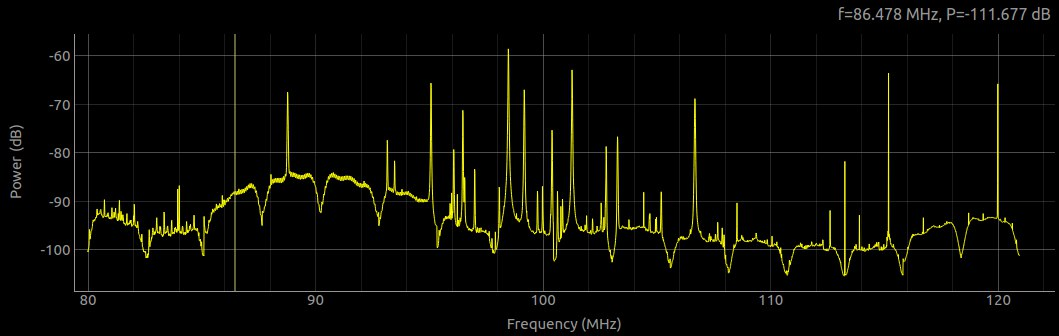
\includegraphics[width=1\textwidth ]
		{Bilder/a3_rtl_sdr.jpg}
		\caption{Hier Caption einfügen}
		\label{fig:Labelx}
\end{figure}

% Als Beispiel wie man referenziert
~\ref{fig:Labelx}

% Beispiel für das Einfügen von Python Code
\begin{python}
print("Hello World")
\end{python}

% Beispiel für das Erzwingen von Abstand 
\hspace{0.5mm}

\end{comment}

\end{document}